\documentclass[a4paper]{article}

\usepackage[T1]{fontenc}
\usepackage[utf8]{inputenc}
\usepackage{gensymb}
\usepackage{pgfplots}
\usepackage{amsmath}
\usepackage{comment}
\usepackage[percent]{overpic}
\usepackage{makecell}
\usepackage{float}
\usepackage{wrapfig}
\usepackage{icomma}
\usepackage{subcaption}
\usepackage{diagbox}
\usepackage{tikz}

% Content of table can have multiple rows
\usepackage{multirow}

% Easily use 1st, 2nd, 3rd etc. in text
\usepackage[super]{nth}

% Indents from sides of paper, etc.
\usepackage[letterpaper]{geometry}
\geometry{verbose,tmargin=1.5cm,bmargin=2cm,lmargin=2cm,rmargin=2cm}

% Graphics operations
\usepackage{graphicx}

% Automatically indent the 1st paragraph in every section
\usepackage{indentfirst}

%  Content divided into multiple columns
%\usepackage{multicol}

% Hypertext links, set their colour and properties
\usepackage{hyperref}
\hypersetup{
colorlinks=true, citecolor=blue, filecolor=blue, linkcolor=blue,
urlcolor=blue
}

\usepackage{listings}
% Code block formatting lstlisting
% 	Usage:
%		\begin{lstlisting}
%			CODE HERE
%		\end{lstlisting}
%% =========================================================

\definecolor{mygreen}{RGB}{28,172,0}
\definecolor{mylilas}{RGB}{170,55,241}
\definecolor{backcolour}{rgb}{0.95,0.95,0.92}

\lstset{language=Matlab}
\lstset{showstringspaces=false}
\lstset{commentstyle=\color{mygreen}}
\lstset{stringstyle=\color{mylilas}}

\lstdefinestyle{myStyle}{
	backgroundcolor=\color{backcolour},
	frame=single,
	keywordstyle=\color{blue},
	morekeywords=[2]{1},
	keywordstyle=[2]{\color{black}},
	identifierstyle=\color{black},
	numbers=left, % Row numbering
	numberstyle={\tiny \color{black}}, % Number font size
	numbersep=9pt, % Number distance from text
	emph=[1]{for,end,break,switch,case,try,catch,arguments},
	emphstyle=[1]\color{blue}, % Colour keywords blue
	basicstyle=\small\ttfamily,
}

\lstset{style=myStyle}

\newcommand{\code}{\texttt}
\usetikzlibrary{positioning}

\linespread{1.2}

% Better math font
\everymath{\displaystyle}

% Larger math font
\DeclareMathSizes{10}{10.5}{9}{9}

% Set the author, institution, date
\newcommand{\Author}{Lukáš Čejka}
\newcommand{\Institute}{FJFI ČVUT v Praze}
\newcommand{\Date}{\today}

\begin{document}

\title{Monte Carlo Method - protocol \\
\textbf{Simulating the spread of COVID-19 using the Monte Carlo method}}
\author{\Author}
\maketitle

% Code in text
\definecolor{codegray}{gray}{0.9}
\renewcommand{\code}[1]{\colorbox{codegray}{\texttt{#1}}}

{
	\hypersetup{linkcolor=black}
	\tableofcontents
}


\section{Introduction}
Whenever a new disease or virus emerges, mankind strives to eliminate, or at the very least, mitigate the negative effect it can have on a human being's health. However, another endeavour is sought after in parallel: minimize the spread. In order to lessen the spread of a virus, one must first understand how it spreads and the speed of reproduction - in the words of the \textit{World Health Organization}: "\textit{The best way to prevent and slow down transmission is to be well informed about the disease and how the virus spreads.}" \cite{WHO2021}. The former can be done via medical analysis, however, the latter relies majorly on statistical data to determine the rate of spread. Concurrently, the collection of data requires time, even more so when it is needs to be statistically significant due to the potential lives at stake. While some initial data may give an embryonic estimate, further analysis can aid in strengthening this understanding. One of many possible ways to analyse such a problem is to visualize it by performing simulations that aim is to replicate the spread of a virus based on a model obtained from real-world data. Recently, Coronavirus has been on the rise with no apparent end in sight, therefore being able to simulate and model the spread of this virus is becoming a discipline of its own when strengthening knowledge around the topic. \\

This protocol aims to replicate the results from \textit{Novel approach for Monte Carlo simulation of the new COVID-19 spread dynamics} \cite{Maltezos2021}, specifically, figures 3 and 4 on page 4 that describe daily new cases and the effective reproductive number in a city, respectively. Similarly to the mentioned paper, MATLAB will be used to implement the simulation. First, section \ref{section:theory} will present a more detailed introduction to the problem and the theory behind the simulation. Then, in section \ref{section:implementation}, the implementation will be described. Last but not least, section \ref{section:results} will contain results obtained from the implementation and their comparison to that of the aforementioned paper. Finally, section \ref{section:conclusion} will encapsulate the summary of this protocol and any further comments.




\section{Theory}\label{section:theory}
In this section, the theory behind the Coronavirus and the simulation methodology will be presented in greater detail.

\subsection{Coronavirus}\label{subsection:coronavirus}
Coronavirus disease (COVID-19) is an infectious disease caused by the SARS-CoV-2 virus \cite{WHO2021}. The name "\textit{Coronavirus}" references reference the similarity of the virus's shape under an electron microscope to that of the solar corona. The virus was discovered towards the end of 2019 in Wuhan, China \cite{Zhou20201203}, however, it is unclear what species the virus originated from with the many scientists suspecting bats. Moreover the means by which the virus spread from animals to humans is a widely debated topic when it comes to specifics.

\paragraph{Symptoms and effects}
Upon being infected with the virus, the majority of people will experience a mild to moderate respiratory illness - akin to pneumonia - and will recover without the need for extensive medical care. On the other hand, some people may require special treatment due a more serious extent of their illness. The symptoms experienced during the progression of the disease are only a part of the problem since many individuals report medical conditions after recovery, for example, limited lung capacity, damaged organs, etc. \cite{MayoClinic22October2021} Among the at-most risk are older individuals, as their underlying conditions (cardiovascular diseases, diabetes, etc.) tend to add to the progression of the disease. Ultimately however, there is no one age group that is safe from becoming seriously ill \cite{WHO2021}.

\paragraph{Virus transmission}
An infectious human can spread the virus via minute liquid particles produced when the person coughs, sneezes, speaks, breathes, etc. - basically, whenever air comes out of a person's mouth and/or nose. The size of one particle ranges from droplets (grains of sand) to much smaller and harder-to-detect aerosols \cite{WHO2021}. Furthermore, once these particles are expelled from an infectious human, they can stay active on surfaces for a number of days. For example, in an indoor environment the virus can survive on non-porous materials for up to 3 days; research differs greatly and the duration depends on the type of surface material, surrounding conditions, viral load etc. - for more information see \textit{Science Brief: SARS-CoV-2 and Surface (Fomite) Transmission for Indoor Community Environments} \cite{CDC5April2021}. The means by which a human can get infected is by absorbing the virus particles via mucous membranes on the eyes, nose, or mouth - this includes inhaling them directly from surrounding air or nearby skin when the human's hand touches a surface with an active virus and then is brought near the aforementioned membranes. The fact that the virus survives on surfaces for prolonged periods of time combined with human nature to subconsciously touch our face and socialize in one way or another results in multiple and simple means of transmission.

\paragraph{Sample case}
Let us consider a sample case where a susceptible human being comes into contact with an infectious human being. First, the susceptible subject is moving around and travelling, or commuting to work, school, shops, etc. In the midst of these commutes the subject can come into contact with an infectious human being. From this point, the subject may or may not develop the disease depending on a number of factors, such as duration of exposure, viral load, immunity strength, etc. Assuming that the subject will eventually developed the disease, it will go through a so-called \textit{incubation period} which lasts until the subject develops symptoms. The most infectious period begins roughly 1-3 days before symptom onset and generally ends 7 days after symptoms appear. Following the infectious period, the subject may experience some symptoms up to 21 days since the exposure - not counting long-lasting post-illness medical conditions. This description is shown in figure~\ref{figure:covid-spread-dynamics} \cite{Maltezos2021}.

\begin{figure}[h!]
	\centering
	\includegraphics{images/covid19_spread_dynamics.jpg}
	\caption{Abstract design showing various time intervals of the virus transmission from an infectious human to another human. The time moments represent mean values. Source: \textit{Novel approach for Monte Carlo simulation of the new COVID-19 spread dynamics} \cite{Maltezos2021}}
	\label{figure:covid-spread-dynamics}
\end{figure}



\subsection{Measured statistics}
The aim of this protocol is reproduce the following statistics from the referenced paper \cite{Maltezos2021}: Daily New Cases (DNC) and the effective reproductive number $R_e$.

\paragraph{DNC}
DNC is simply the number of newly infected human beings on a given day.

\paragraph{Effective reproductive number}
The effective reproductive number is one of two numbers associated with determining disease spread speed in epidemic theory. It is defined as \textit{the average number of secondary cases per infectious case in a population made up of both susceptible and non-susceptible hosts} \cite{Barratt2018}. If $R_e > 1$, then the number of cases will increase - start of epidemic. If $R_e = 1$, then the disease is endemic, which in the instance of Coronavirus means that it is not spreading. If $R_e < 1$ then there will a decline in the number of cases \cite{Barratt2018}. While there is no one single formula defining this number, the authors of the reference paper \cite{Maltezos2021} used the definition listed in equation~\ref{equation:effective-reproductive-number}

\begin{equation}
	R_e = 1 + \ln\left(\frac{I_{t_i}}{I_{t_{i-1}}}\right)^\frac{1}{c}
	\label{equation:effective-reproductive-number}
\end{equation}
\noindent
where $I_{t_i}$ represents the number of infectious cases at time $t_i$ and $c$ can be considered a constant that differs slightly from 1, however, in practice it does not have a significant impact on the result, therefore for the purpose of this protocol it was set as 1.



\subsection{Simulation methodology}\label{subsection:simulation-methodology}
The simulation of the spread of Coronavirus in this protocol is built on a \textbf{SIR}-based model which is often used in mathematical modelling of infectious diseases as it divides a specific population of humans (e.g. a city, country, or just a group of humans) into labelled compartments:
\begin{itemize}
	\item \textbf{S}usceptible - humans that are susceptible to the infection.
	\item \textbf{I}nfectious - humans that are currently infectious and able to spread the disease.
	\item \textbf{R}ecovered/\textbf{R}emoved - humans that have either recovered or died (removed from simulation) and therefore cannot be infected and cannot infect again. 
\end{itemize}

When it comes to simulating the behaviour described in section~\ref{subsection:coronavirus}, it is paramount to include only processes that have an impact on the results. The aim of this protocol is to reproduce the Daily New Cases (DNC) and effective reproductive number $R_e$, as was stated in the introduction. For both of the monitored statistics, there are certain aspects of the sample case that need not be accounted for, e.g., dividing time intervals related to the health status of the human subject. The only health status needed for the purpose of simulating the spread of the virus is when the human is infectious, as it is during this period that the subject can infect susceptible humans. Therefore the only remaining aspects that ought be an integral part of the simulation are:
\begin{itemize}
	\item Daily movement - \nth{1} part of the sample case. The human subject travels and commutes (random process).
	\item Physical distance - \nth{2} part of the sample case. The human subject is exposed to an infectious human being (random process).
	\item Infectious period - \nth{3} part of the sample case. The human subject is sick for a specific time period (random process).
\end{itemize}

\paragraph{Daily movement}
During their daily lives, human beings majorly follow a predictable routine on an individual level. However, when trying to generalize the movement for an average human, there is simply no other way than to create some sort of random process. In the case of daily movement, there are two random processes to consider: direction and length of step. The former will follow a uniform distribution on a unit circle and the latter a Gaussian distribution. Thus, for the purpose of this simulation, every human subject will move in a random direction with a random step length. However, it needs to be mentioned that the reference paper \cite{Maltezos2021} only specifies the random distribution of the step length, i.e., it does not mention what distribution the direction of daily movement should follow.

\paragraph{Physical distance}
During their daily movement, human beings can come into contact with other human beings, some of whom may be infectious (this simulation does not consider quarantining human beings). As mentioned before, in real life multiple variables contribute to the successful transmission of a virus. The simulation of each combination was not considered in the reference paper \cite{Maltezos2021}, therefore, they will be aggregated into physical distance. Let there be two human beings. One of whom is infectious and the other susceptible. Therefore, the probability of the virus being transmitted from the infectious human to the susceptible human is a random variable solely based on the physical distance between the two humans. As in the reference paper \cite{Maltezos2021}, this random process will follow the Exponential distribution. See equation~\ref{equation:exp-distr} for the PDF of the exponential distribution

\begin{equation}
	f(x,\:\lambda) = \lambda e^{-\lambda x}
	\label{equation:exp-distr}
\end{equation}
\noindent
where $x > 0$ is a random variable and $\lambda$ is the rate parameter.

\paragraph{Infectious time}
Following the exposure of a susceptible human subject to the virus and a subsequent transmission of the virus, the subject becomes infectious. Since every human being is different when it comes to immunity strength and other factors that dictate how long the subject will be infectious for, it is assumed that the duration of the subject's infectiousness is a random variable from the Gamma distribution. See equation~\ref{equation:gamma-distr} for the PDF of the Gamma distribution

\begin{equation}
	f(x,\:\alpha,\:\beta) = \frac{\beta^\alpha}{\Gamma \left(\alpha\right)} x^{\alpha-1} e^{-\beta x}
	\label{equation:gamma-distr}
\end{equation}
\noindent
where $x > 0$ is a random variable, $\alpha$ is the shape parameter and $\beta$ is the rate parameter.




\section{Implementation}\label{section:implementation}
In this section, the simulation setup will be described along with examples of code.

\subsection{Simulation setup}
The simulation setup of the SIR model can be divided into two parts: constants and random processes.

\subsubsection{Constants}
The constants of the simulation revolve mainly around the city. In the reference paper \cite{Maltezos2021}, the authors specify that their model aims to simulate the spread of the Coronavirus in a city with a given population density. However, there are additional constants - indirectly mentioned in the paper - that need to be accounted for, e.g., the number of days the simulation should run, whether humans are allowed to escape the city bounds and the distribution of humans' starting positions within the city. Table~\ref{table:simulation-configuration} specifies the simulation configuration for this protocol.

\begin{table}[!h]
	\centering
	\begin{tabular}{ |l|r|l|  }
		\hline
		Property name & Property value [units] & Mentioned in reference paper \\
		\hline
		\hline
		City dimensions               & 1000 x 1000 [m]                 & Indirectly \\
		City population               & 2000 [humans]                   & Indirectly \\
		Population density            & 2000 [humans/$\textrm{km}^2$]   & Yes \\
		Initial infectious population & 0.5 [\%]                        & Yes 	  	 \\
		Length of simulation          & 100 [days]                      & Indirectly \\
		Humans constrained in city    & Yes                             & No         \\
		\hline
	\end{tabular}
	\caption{Properties of the simulation configuration and their values, along with a column specifying whether the property is mentioned in the reference paper \cite{Maltezos2021}.}
	\label{table:simulation-configuration}
\end{table}

In summary, the modelled city in the shape of a $1000\:\textrm{x}\:1000\textrm{m}$ ($1\: \textrm{km}^2$) square will house a population of 2000 people of which 10 (0.5\%) are infectious since the genesis of the simulation. By default, humans are constricted to the city bounds and the spread of the virus will be simulated over the course of 100 days. For reference, larger cities (e.g., Paris and Mumbai) have a population density of up to 20 000 people per $\textrm{km}^2$ \cite{GnfKtXcXYiGm8NmR}\cite{YyQLmGbzBu9Drxx5}.


\subsubsection{Random processes}
In this part all random processes explained in subsection \ref{subsection:simulation-methodology} will be specified - specifically the parameters of their respective distributions that were selected by the authors of the reference paper \cite{Maltezos2021} as they present characteristics consistent with their respective properties when it comes to medical observations.

\paragraph{Daily movement}
The daily movement of a human being in one day of the simulation utilizes two random variables: angle (direction) of movement and the length of the step. The angle follows a uniform distribution on a unit circle, in other words, all directions have the same probability of being selected, in theory. The step length (length of movement) follows the Gaussian (Normal) distribution with a mean step equal to $1/48$ of the city dimensions and a standard deviation equal to 1/144 of the city dimensions. These values were chosen differently than specified in the reference paper as they best recreate the results in the reference paper \cite{Maltezos2021}. If the values specified in the reference paper \cite{Maltezos2021} are followed exactly, then a human being would either have a mean step equal to $2\:\textrm{m}$ a day or $250\:\textrm{m}$ a day in a $1000\:\textrm{x}\:1000\:\textrm{m}$ city - depending on the interpretation (see the \nth{1} bullet point in section \textit{2. Simulation methodology} of the reference paper \cite{Maltezos2021}).\\
In the implementation accompanied by this protocol, the new location of a human is generated with respect the human's current position using Polar coordinates and then converted to Cartesian coordinates.

\paragraph{Physical distance}
The probability of infection given a distance between and infectious human being and a susceptible human being follows the Exponential distribution. There are two parameters listed in equation~\ref{equation:exp-distr}: $\lambda$ and $x$. The mean value is equal to $1/\lambda$ which in this simulation is equal to $8\:\textrm{m}$. The distance between humans $x$ is assumed positive. The probability of infection can be obtained by integrating Exponential distribution's PDF from the distance to infinity:

\begin{equation}
	\int_{x}^{\infty} \lambda e^{-\lambda u} \,du = e^{-\lambda x} 
\end{equation}
\noindent
For example, given two humans - one infectious and one susceptible - $2\:\textrm{m}$ apart, the probability of the susceptible humans being infected is equal to

\begin{equation}
	e^{- \frac{2}{8}} = 0.7788
\end{equation}
\noindent
in other words, 78\%.

\paragraph{Infectious period}
The infectious period of a human being is a random process following the Gamma distribution, where $x > 0$ is a random variable, the mean value is $\mu = \alpha/\beta$ and the variance $ \sigma^2 = \alpha/\beta^2$. Similarly to the reference paper \cite{Maltezos2021}, $\alpha = 6$ and $\beta = 2/3$ days making the mean infectious period 9 days and the square root variance equal to 4.9 days.



\subsection{Code examples}
The simulation was implemented purely in MATLAB as it already houses many functionalities required for this project along with simple visual output of results. Even though MATLAB benefits heavily from vectorization, the simulation class structure was designed with an object-oriented approach using handle classes to assure ease of readability and serve as practice when it comes to software development. The class structure can be seen in figure~\ref{figure:simulation-class-diagram}. It can be seen that the main driving class is \code{simulation}, which houses the \code{city} class where the simulation will take place, the \code{configuration} class where the simulation configuration is stored and finally, the \code{data} class where all data related to the simulation is stored, processed and outputted.

An example of the process of determining newly infected humans on a given day can be seen in code blocks \ref{code:simulate-day}, \ref{code:update-health-status}, \ref{code:update-infectious}, \ref{code:infect-susceptible-humans}, \ref{code:get-infection-prob-of-human}.

\begin{lstlisting}[caption={Function for simulating one day, where \code{obj} is \code{city}.}, captionpos=b, label={code:simulate-day}]
function simulate_day(obj, day)	
  obj.population.update_health_status(day);
  obj.population.update_humans(day);
	
  for human = obj.population.humans_by_status.all
    human.move_to_random_position()
  end
end
\end{lstlisting}


\begin{lstlisting}[caption={Function for updating the health status of the population on a given day, where \code{obj} is \code{population}.}, captionpos=b, label={code:update-health-status}]
function update_health_status(obj, day)		
  obj.update_infectious(day);
  obj.update_recovered(day);
end
\end{lstlisting}

\begin{lstlisting}[caption={Function for updating infectious humans, i.e., deciding which susceptible humans will every infectious humans infect, on a given day, where \code{obj} is \code{population}.}, captionpos=b, label={code:update-infectious}]
function update_infectious(obj, day)
  for human = obj.humans_by_status.infectious
    human.infect_susceptible_humans(day, obj.humans_by_status.susceptible);
  end
end
\end{lstlisting}

\begin{lstlisting}[caption={Function for infecting susceptible humans by an infectious human on a given day, where \code{obj} is \code{human} - specifically, an instance of \code{human} whose health status is infectious.}, captionpos=b, label={code:infect-susceptible-humans}]
function infect_susceptible_humans(obj, day, susceptible_humans)
  for susceptible_human = susceptible_humans                
    infection_prob = obj.get_infection_prob_of_human(susceptible_human);

    if rand() <= infection_prob
      susceptible_human.set_health_status('infectious', day=day);
    end
  end                
end
\end{lstlisting}

\begin{lstlisting}[caption={Function for getting the probability of infection between an infectious human and a susceptible human, where \code{obj} is \code{human} - specifically, an instance of \code{human} whose health status is infectious.}, captionpos=b, label={code:get-infection-prob-of-human}]
function prob = get_infection_prob_of_human(obj, human)		
  distance = obj.get_eucledian_distance_from_human(human);
  prob = round(exp(-distance/obj.infection.mean_distance), 2);
end
\end{lstlisting}

\begin{figure}[h!]
	\centering
	\includegraphics[scale=0.65]{images/simulation_class_diagram.png}
	\caption{Class diagram for the simulation, where black lines represent connections between class properties and classes. For example, the \code{simulation} class contains properties: \code{city}, \code{config} and \code{data}, all of which represent instances of classes \code{city}, \code{configuration} and \code{data}, respectively.}
	\label{figure:simulation-class-diagram}
\end{figure}




\section{Results}\label{section:results}
Results obtained from the simulation can be seen in figure~\ref{figure:results-protocol} and the results from the reference paper \cite{Maltezos2021} can be found in figure~\ref{figure:results-reference-paper}.
\par
When comparing DNC results, it can be seen that the trend is comparable with both simulations exhibiting a sharp rise in cases from the beginning until 15-20 days into the simulation. Moreover, the gradual lessening of daily new cases eventually becomes zero about 50-60 days into the simulation - with minor deviations.

\par
When comparing results of the effective reproductive number, we can see that there are error bars present in figure~\ref{figure:rp-r-e}, however, they appear to be missing in figure~\ref{figure:results-r-e}. This is due to the fact that the authors in the paper do not clearly explain what these error bars represent - reproductive efforts for this indicator failed. Nevertheless, data obtained from the simulation seems to correspond to the trend obtained from the reference paper \cite{Maltezos2021} with some minor differences. The main difference stems in the minimum and maximum values, which in the case of the reference paper \cite{Maltezos2021} almost seem to have been calculated using a different formula than what the one found in equation~\ref{equation:effective-reproductive-number}. The main indicator for this reasoning is that The initial values for $R_e$ reach a maximum of 3, which would mean that the number of cases should have tripled in the first 5-6 days, which according to figure~\ref{figure:rp-dnc} does not seem to be the case. For reference, in order achieve the same initial $R_e$, the mean infection distance needs to be tripled in the simulation. Nonetheless, the overall rising and declining characteristics of the effective reproductive number are pertinent between the two simulations.

\begin{figure}[h!]
	\centering
	\begin{subfigure}{.5\textwidth}
		\centering
		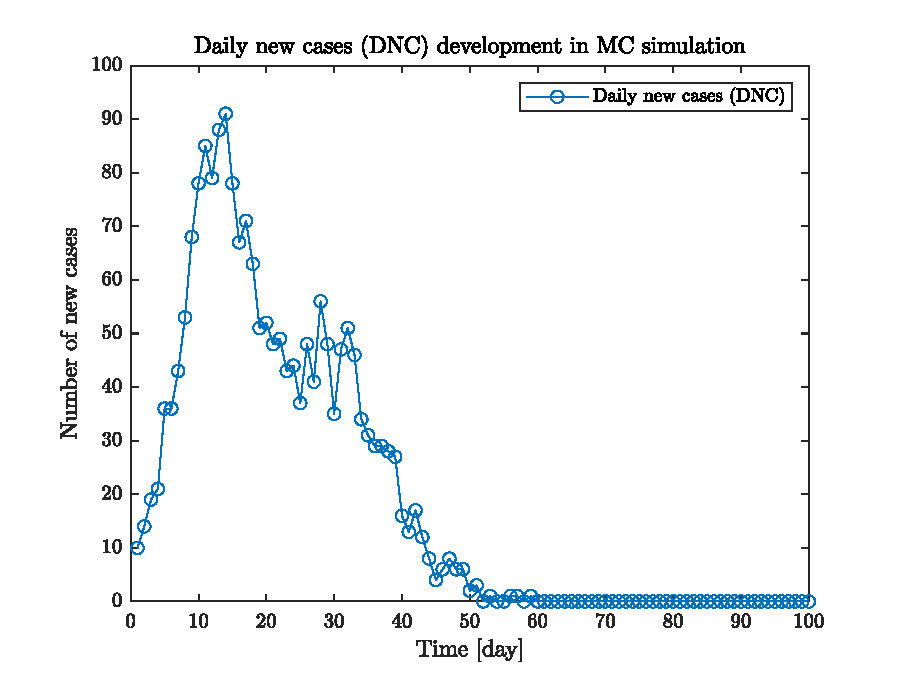
\includegraphics[width=\textwidth]{images/dnc.eps}
		\caption{Daily new cases}
		\label{figure:results-dnc}
	\end{subfigure}%
	\begin{subfigure}{.5\textwidth}
		\centering
		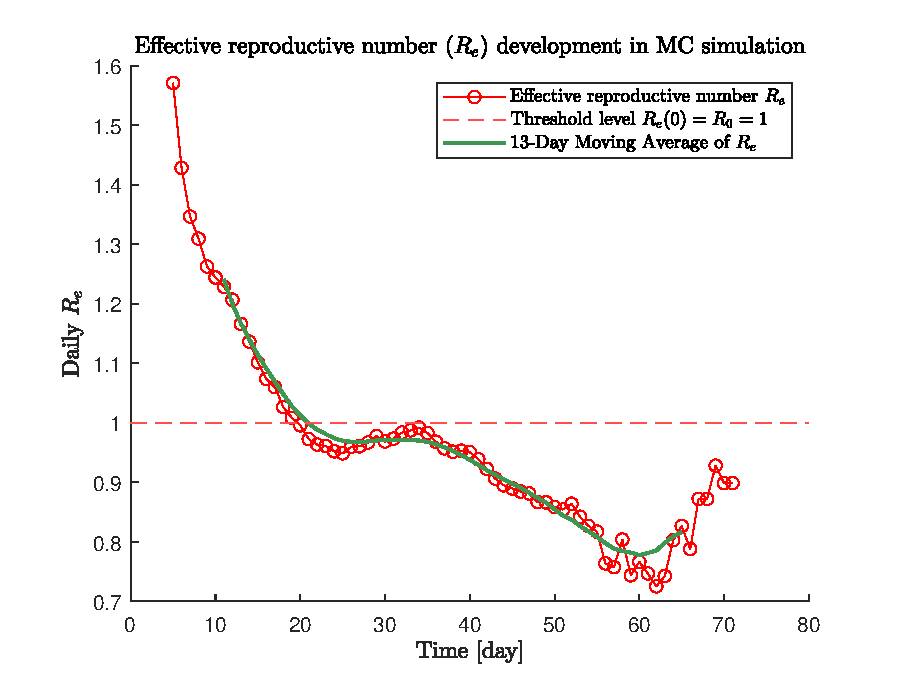
\includegraphics[width=\textwidth]{images/r_e.eps}
		\caption{Effective reproductive number}
		\label{figure:results-r-e}
	\end{subfigure}
	\caption{Graphs depicting the daily new cases and the effective reproductive number obtained from the simulation.}
	\label{figure:results-protocol}
\end{figure}

\begin{figure}[h!]
	\centering
	\begin{subfigure}{.5\textwidth}
		\centering
		\includegraphics[width=\textwidth]{images/dnc-orig.jpg}
		\caption{Daily new cases}
		\label{figure:rp-dnc}
	\end{subfigure}%
	\begin{subfigure}{.5\textwidth}
		\centering
		\includegraphics[width=\textwidth]{images/r_e-orig.jpg}
		\caption{Effective reproductive number}
		\label{figure:rp-r-e}
	\end{subfigure}
	\caption{Graphs depicting the daily new cases and the effective reproductive number obtained from the reference paper \cite{Maltezos2021}.}
	\label{figure:results-reference-paper}
\end{figure}




\section{Conclusion}\label{section:conclusion}




\bibliographystyle{IEEEtran}
\bibliography{references/references} 

\end{document}